\documentclass[12pt]{article}
\usepackage{listings}
\usepackage[usenames,dvipsnames]{color}  
\usepackage{titlesec}      
\usepackage{amsmath}
\usepackage{amsfonts}
\usepackage{amssymb}
\usepackage{pdfpages}
\usepackage{graphicx}
\usepackage{listings}
\usepackage{caption}
\usepackage{proof}
\usepackage{tabularx}
\usepackage{xcolor}
\usepackage{titlesec}
\usepackage{rotating}
\usepackage{float}
\usepackage{tikz}
\usepackage{hyperref}
\usepackage{fontspec} % LuaTeX compatible font package
\usepackage[left=2cm,right=2cm,top=2cm,bottom=2cm]{geometry}

\usepackage[style=ieee]{biblatex}
\addbibresource{refs.bib}

\captionsetup{labelfont={small,bf}, textfont=small}

\renewcommand*\thesection{\arabic{section}}
\renewcommand{\familydefault}{\sfdefault}

\titleformat{\section}{\fontsize{13pt}{15pt}\bfseries}{\thesection}{1em}{}
\titleformat{\subsection}{\fontsize{13pt}{15pt}\bfseries}{\thesubsection}{1em}{}
\titleformat{\subsubsection}{\fontsize{13pt}{15pt}\bfseries}{\thesubsubsection}{1em}{}

\setmainfont{Carlito}

\graphicspath{ {./plots/} }

% Depth for table of contents and section numbering
\setcounter{tocdepth}{4}
\setcounter{secnumdepth}{4}
        
% Define colors for listings
\definecolor{dkgreen}{rgb}{0,0.6,0}
\definecolor{gray}{rgb}{0.5,0.5,0.5}
\definecolor{mauve}{rgb}{0.58,0,0.82}

% Set paragraph formatting
\setlength{\parindent}{0pt}
\setlength{\parskip}{6pt}

% Load TikZ libraries
\usetikzlibrary{automata,positioning}
\tikzstyle{every state}=[fill={rgb:black,1;white,10}]


\begin{document}
\newpage
\subsection*{2. Background}
\subsubsection*{2.? Logistic Regression}
Logistic regression is a supervised machine learning model, a variant of the linear regression model in which the outcome variable is dichotomous~\cite{Hosmer2013}. Unlike linear regression, logistic regression is used for classification, in which the model finds the boundary line of the classification between the two classes~\cite{Zou2019}. This is represented by the conditional probability \(P(Y|X)\) where \(X\) is a real number (input features) and the random variable \(Y\) takes the value of 1 or 0~\cite{Li2024}. The input variable \(X\) can be desribed as a set of features \((x_0, x_1, x_2, ..., x_n)\) which are multiplied by a set of associated weights \((w_0, w_1, w_2, ..., w_n)\), and summed together to produce the dot product~\cite{Zou2019}. Therefore:

\[z = w_{0}x_{0}+ w_{1}x_{1} + w_{2}x_{2} + ... + w_{n}x_{n}\]
\[z = w \cdot x = w^{T}x\]

This is then passed to a function which converts \(z\) to a value between 0 and 1. The Sigmoid function is the most widely used function for this~\cite{Zou2019}, and the distribution is shown in Figure~\ref{fig:sigmoid}. The Sigmoid function is given by:

\[\sigma(z) = \frac{1}{1 + e^{-z}}\]

\begin{figure} [H]
  \centering
  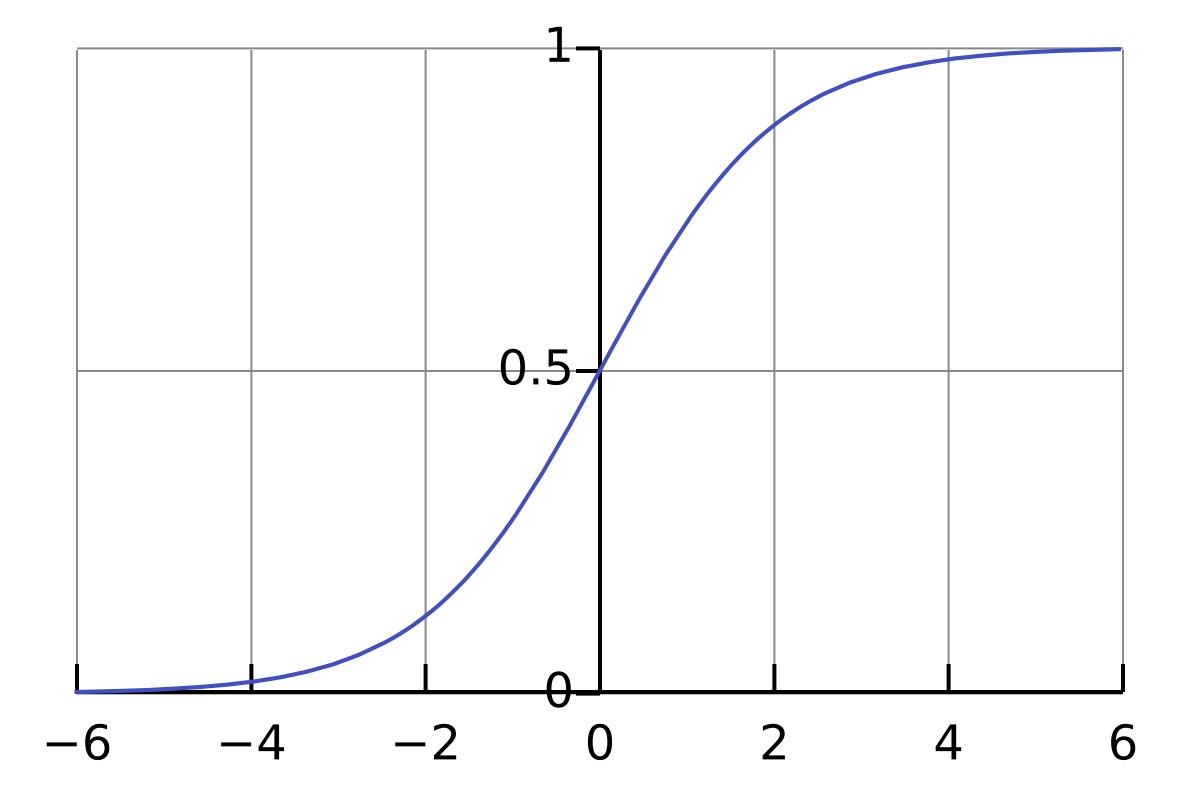
\includegraphics[width=0.7\linewidth]{sigmoid}
  \caption{Sigmoid function.}\label{fig:sigmoid}
\end{figure}  


After being passed through the Sigmoid function, the data point is then given the prediction of belonging to the class 0 or 1. Therefore, if \(\sigma(w^{T}x) \geq 0.5\) then the outcome is class 1, and if \(\sigma(w^{T}x) < 0.5\) then the outcome is class 0. The weights of the logistic regression model are found during training the model using Maximum Likelihood Estimation (MLE) as the cost function~\cite{Li2024}.

While standard logistic regression gives a binary outcome variable, it can also be used for multi-class problems. This is done using techniques such as one-vs-rest (OvR) \textbf{Other techniques? Find source}. The one-vs-rest model trains separate binary classifiers for each class, with each classifier distinguishing one class from the rest. 

\newpage
\subsection*{3. Data Preparation}
\subsubsection*{3.1. Exploratory Analysis}
The initial dataset consisted of 4424 records with 36 independent variables, with no missing values. The dataset was processed using the \textit{pandas} library in Python.

\begin{itemize}
    \item{\textbf{Note: Should I include means of variance tables despite not all variables being in the final MI dataset?}}
\end{itemize}

Each student entry has one of 3 Target variables: Graduated, Dropout, or Enrolled (where the student took another three years to complete the course). The distribution of the Target variable is shown in Figure~\ref{fig:target}, which shows that it is imbalanced, where the Graduated Target makes up 50\% of the data records. This was addressed using the Synthetic Minority Over-sampling Technique (SMOTE), an oversampling algorithm which generates synthetic data using \textit{k} nearest neighbours~\cite{smote}. The SMOTE implementation from \textit{imbalanced-learn} in the \textit{sci-kit learn} library was used.

\begin{figure} [H]
    \centering
    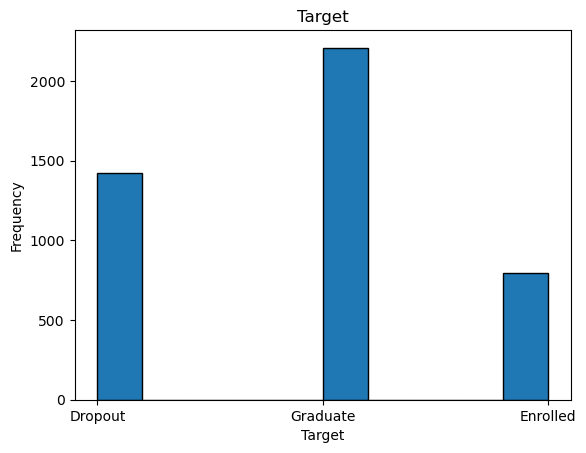
\includegraphics[width=0.8\linewidth]{target_plot}
    \caption{Count of Target variable.}\label{fig:target}
  \end{figure}  

\subsubsection*{3.2. Feature Engineering}

Mutual Information (MI) is a filter-based feature selection method which measures how mutually dependent two variables are~\cite{VenkateshAnuradha2019}. This method was used to filter out redundant variables, and was opted for since MI can be used for both discrete and continuous variables. The MI score with target was computed for each variable using \textit{sci-kit learn}. Each feature is assigned a scoring value, with the resulting features being organised in descending order based on the scores and are assigned rankings for the features~\cite{VenkateshAnuradha2019}. A limitation of this method is that while it measures a feature's importance by it's correlation with the target, it assumes independence of features from each other~\cite{Li2017}. Therefore, choosing the highest scoring variables from MI can lead to redundant features can be selected.

To address this, a pairwise MI matrix was computed. The values were normalised to a range between 0 and 1, presented in Figure~\ref{fig:pairwise_mi}. Redundant variables were removed by checking each MI pairwise score according to a set threshold (0.99) and removing the variable with the lower MI score with the target. The final selected predictors resulted in 17 independent variables.

\begin{figure} [H]
    \centering
    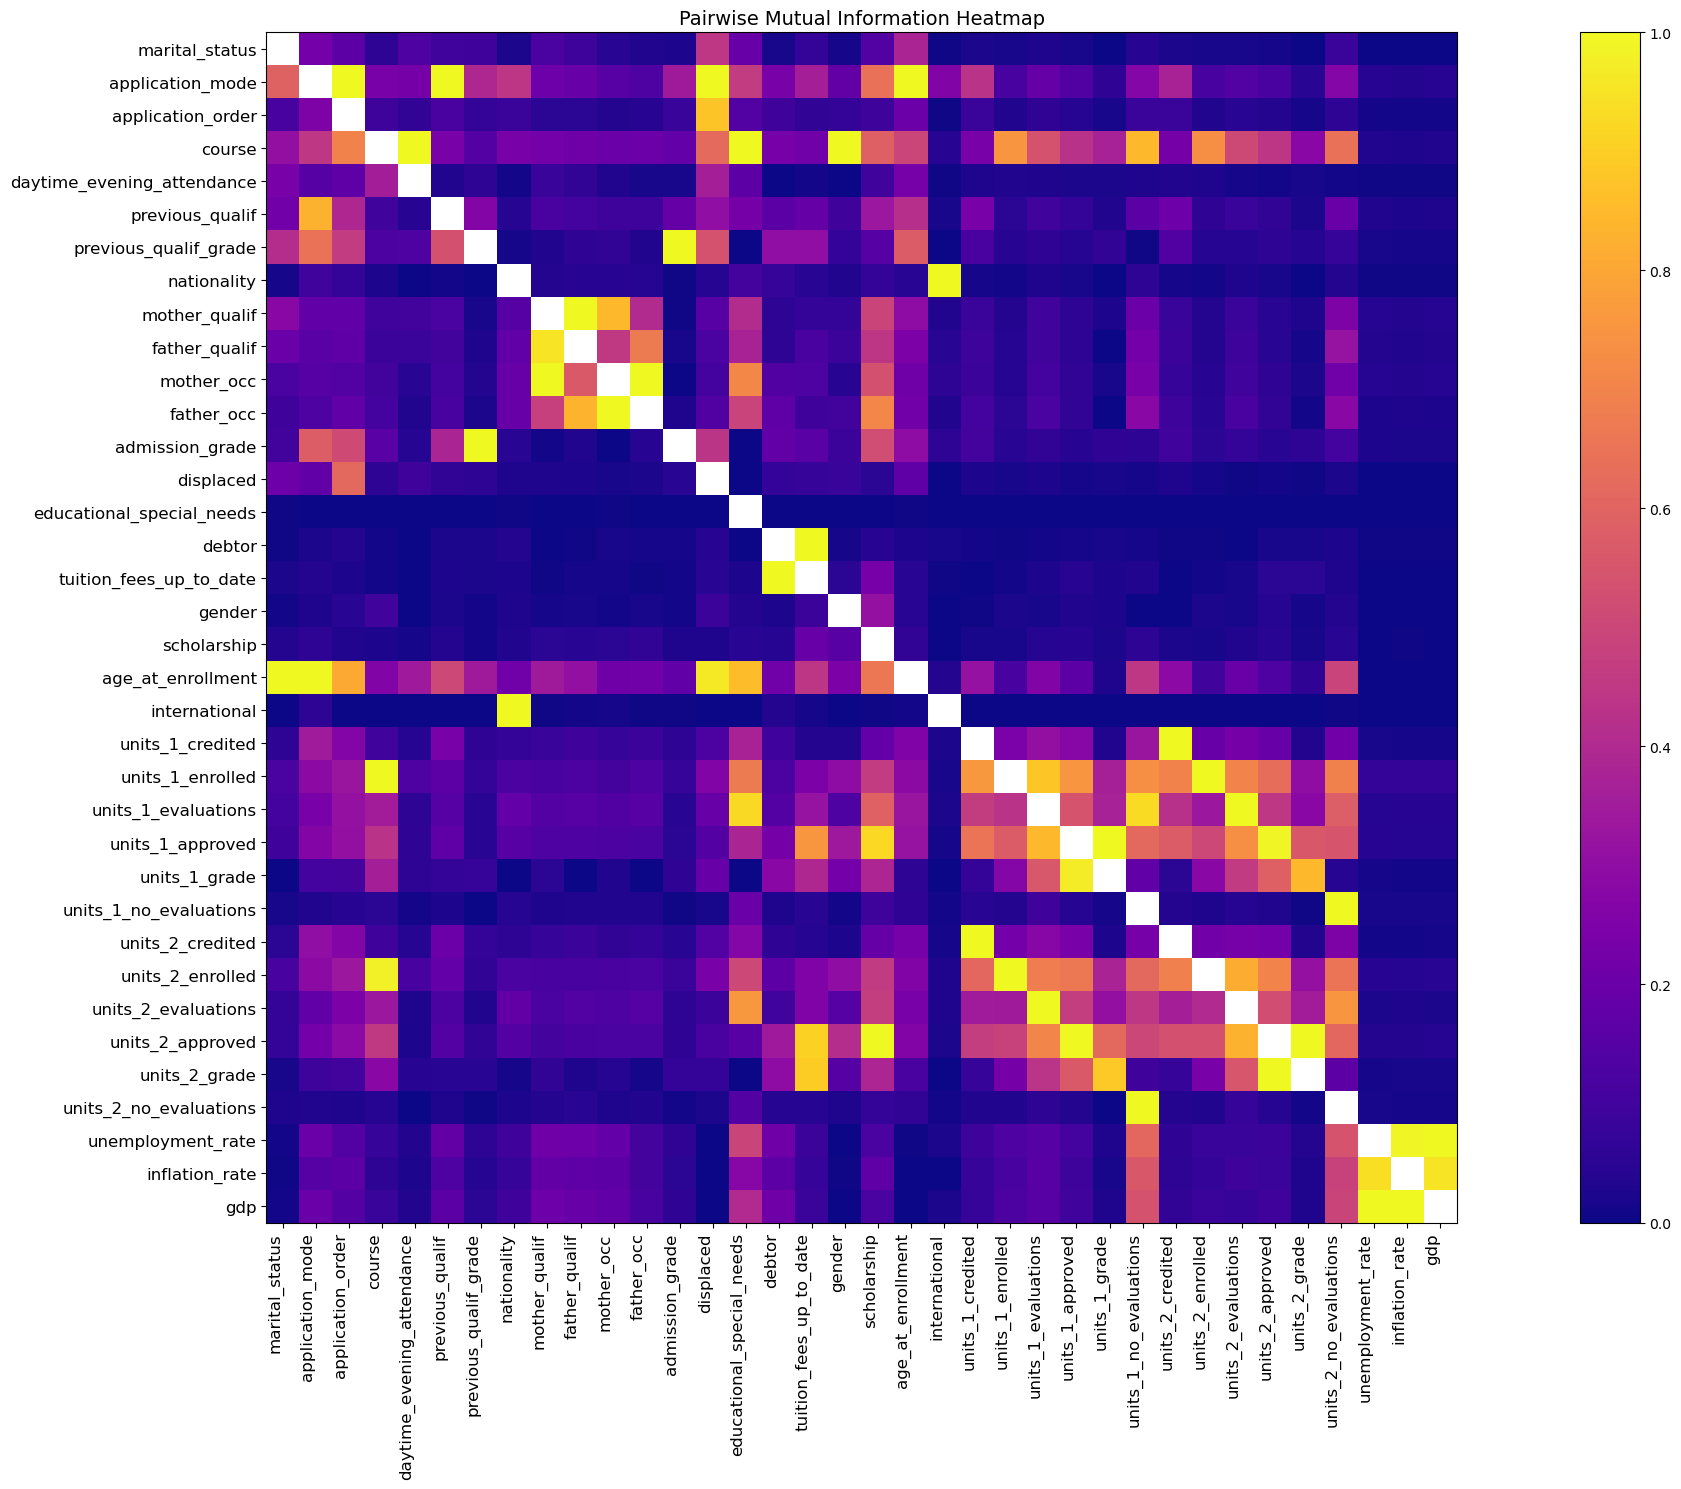
\includegraphics[width=0.8\linewidth]{pairwise_mi}
    \caption{Heatmap of pairwise Mutual Information scores.}\label{fig:pairwise_mi}
  \end{figure}  

Principal Component Analysis (PCA) was then performed on the dataset for dimensionsality reduction~\cite{Gewers2021}. \textbf{Explain PCA briefly.} The final resulting dataset consisted of 8 independent variables.

\newpage
\subsection*{4. Experiments}
\subsubsection*{4.? Logistic Regression}

The multi-class logistic regression model was implemented using the \textit{sci-kit learn} library in Python. The dataset was split into training, validation, and test sets using a 70/20/10 split to ensure that the model was trained on a representative sample and tested on unseen data. Feature scaling was applied using \textbf{StandardScaler?} to ensure that the coefficients of the logistic regression were appropriately scaled.

\textbf{The LogisticRegression class was utilised - 'multinomial' option? OvR or cross-entropy loss?} \textbf{Solver lbfgs}. Model evaluation was performed on the test set using metrics the accuracy, precision, recall, F1-score metrics, and a confusion matrix to assess classification performance. The \textit{scikit-learn} classification\_report and confusion\_matrix functions were used for this. 

Table~\ref{tab:logist_results} shows the results of the classification report and Figure~\ref{fig:logist_confusion} shows the confusion matrix. The overall model accuracy is 61\%. Results show that the Dropout target has the highest Precision and F1-Scores, indicating that the model has the best results for predicting this class over others. The model struggles most in predicting the Enrolled target, with an F1-score of 0.54.
 
\begin{table}[h!]
  \centering
  \begin{tabular}{ | m{2.5cm} || m{2cm} | m{2cm} | m{2cm} | } 
    \hline
    \textbf{Target} & \textbf{Precision} & \textbf{Recall} & \textbf{F1-Score} \\ 
    \hline
    \hline
    \textbf{Graduate} & 0.61 & 0.59 & 0.60 \\ 
    \hline
    \textbf{Dropout} & 0.74 & 0.67 & 0.70 \\ 
    \hline
    \textbf{Enrolled} & 0.51 & 0.57 & 0.54 \\
    \hline
  \end{tabular}
  \caption{Classification report for Logistic Regression model.}
  \label{tab:logist_results}
\end{table}

\begin{figure} [H]
  \centering
  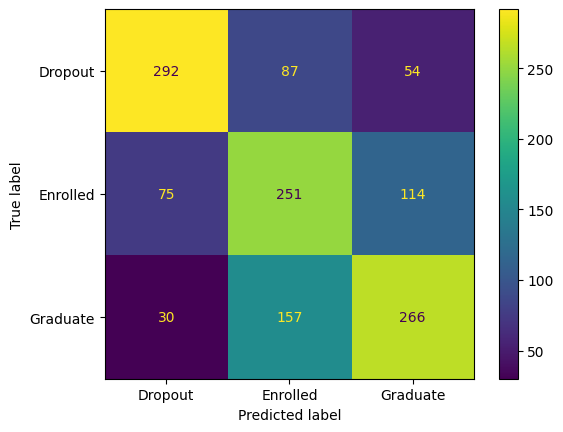
\includegraphics[width=0.8\linewidth]{logist_confusion}
  \caption{Confusion Matrix of the Logistic Regression model.}\label{fig:logist_confusion}
\end{figure}  

\printbibliography[heading=bibintoc, title={References}]
\end{document}